\chapter{Modellazione della deambulazione}
Il lavoro svolto, pu� essere suddiviso in tre fasi principali: 
\begin{enumerate}
	\item \textbf{Creazione ed addestramento di un modello}: scelta di un modello consono al problema e ottimizzazione dei relativi parametri,
	\item \textbf{Sviluppo applicazione}: implementazione di un programma per \textit{Smartphone} Android\tm 	del modello,
	\item \textbf{Valutazione delle prestazioni dell'applicazione in condizioni di uso reali}: il sistema ottenuto � stato valutato correlando un parametro spaziale del cammino (la distanza percorsa) a partire da quelli temporali ottenuti con la segmentazione (cadenza e velocit�) e successivamente verificandone la correttezza con misurazioni dirette dei parametri spaziali tramite GPS (\textit{Global Positioning System}) sistema di posizionamento globale.
\end{enumerate}

\section{Raccolta dati}
Sono stati scelti 6 soggetti sani (con deambulazione normale) e sono stati sottoposti a 5 sessioni di cammino e 5 sessioni di corsa.
Le prove sono state compiute su un tappeto rullante con pendenza 0�, nell'intervallo di velocit� [3-7]Km/h per il cammino e [8-12]Km/h per la corsa. La prima sessione alla velocit� di 3Km/h e con un incremento di 1Km/h in ciascuna sessione successiva. Ciascuna sessione � stata della durata di 2 minuti.

\begin{table}[htbp]
	\centering
	\begin{tabular}{|l|c|c|}
		\hline		
			\textbf{Attivit�}& cammino & corsa \\
			\hline
			\textbf{Soggetti}& 6 & 5\\
			\hline
			\textbf{Velocit�}& \{3,4,5,6,7\}Km/h & \{8,9,10,11,12\}Km/h\\
			\hline
			\textbf{Durata}& \multicolumn{2}{c|}{2 minuti per attivit�}\\
			\hline
			\textbf{Strumenti} & \multicolumn{2}{c|}{IMU, Vicon, tappeto rullante}\\
			\hline
			\textbf{Luogo}& \multicolumn{2}{c|}{Laboratorio}\\
			\hline
			\textbf{Dati raccolti} & \multicolumn{2}{c|}{valori giroscopio monoassiale}\\
			\hline
			\textbf{Frequenza campionamento} & \multicolumn{2}{c|}{100 Hz}\\
			\hline
		\end{tabular}
	\caption{Tabella riassuntiva della raccolti dati}
	\label{tab:TabellaRiassuntivaRaccoltaDati}
\end{table}

Le sessioni sono state tutte eseguite posizionando saldamente una IMU (vedi appendice \ref{sec:sensori}) sul collo del piede dei soggetti mediante un cinturino in velcro. Il tipo di sensore usato � un giroscopio monoassiale (Murata ENC-03J) con asse di sensibilit� orientato sul piano mediale-laterale (sagittale) (vedi figura \ref{fig:HumanBodySPL}).\\
I segnali sono stati campionati dal sensore ad una frequenza di 100 Hz e filtrati mediante un filtro passa-basso\footnote{Un filtro elettronico nella Teoria dei Segnali � un circuito elettronico che riceve dei segnali in ingresso e li trasforma secondo un criterio. Un filtro passa-banda (banda alta o banda bassa) lascia passare segnali a frequenza in un intervallo scelto mentre blocca il passaggio (o le attenua) il passaggio di segnali fuori dall'intervallo. Un filtro passa-basso quindi lascia passare le frequenze basse, e smorza quelle a frequenze alte.} a 15Hz mediante un filtro ricorsivo \textit{forward-backward}(Fw-Bkw)\footnote{Un filtro ricorsivo riusa i propri valori in uscita come ingresso. In particolare un filtro Fw-Bkw � un filtro ricorsivo che viene utilizzato per avere un segnale simmetrico.} di \textit{Buttersworth}\footnote{Filtro detto "`massimamente piatto"', perch� non solo rifiuta i segnali a frequenze non desiderate, ma ha la stessa sensibilit� per tutte le frequenze desiderate.}. 
Dai dati raccolti, quelli considerati per lo studio sono quelli compresi nell'intervallo dai 50 ai 110 secondi. \\

\begin{figure}
	\centering
		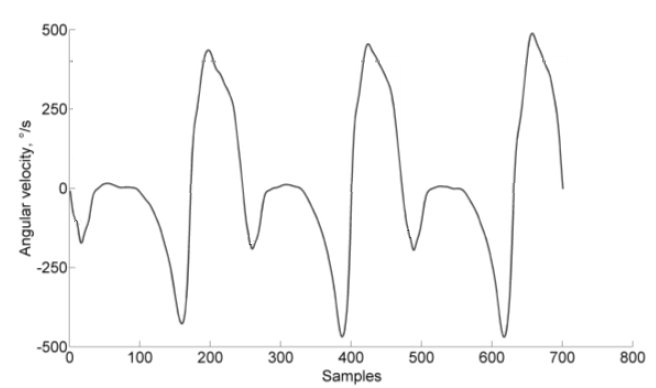
\includegraphics[width=1\textwidth]{imgs/patternGyro.jpg}
	\caption{Grafico del segnale di un giroscopio posizionato sul piede.}
	\label{fig:gyroPattern}
\end{figure}

Il grafico del segnale del giroscopio posizionato sul piede ha una struttura definita e ripetitiva (vedi grafico \ref{fig:gyroPattern}). Nel grafico, l'ascissa rappresenta i campioni e l'ordinata la velocit� angolare in gradi al secondo (�/s). La forma del grafico pu� essere descritta a grandi linee come un picco negativo seguito da un tratto quasi orizzontale ed un secondo picco negativo ed uno positivo. Tale sequenza rappresenta un passo completo e si ripete quasi identica a se stessa durante la camminata.


\section{Modello: HMM}
Il modello di deambulazione scelto � di tipo stocastico una HMM sinistra-destra ad emissioni continue (vedi appendice \ref{sec:tipi_hmm}). Questa rappresenta il susseguirsi degli intervalli tra gli eventi della deambulazione. 
In dettaglio l'HMM � stata definita nel seguente modo:
 \begin{equation}
	Deamb\_HMM = <N, M, \mathbf{A}, \mathbf{B}, \pi>
\label{eq:deamb_hmm}
\end{equation}
dove:
 \begin{enumerate}
	\item $N = 4$ � la cardinalit� dell'insieme degli stati $S = \{HS, FF, HO, FO\}$. Gli stati corrispondono agli intervalli fra un evento ed il successivo come mostra la tabella \ref{tab:4_fasi_deambulazione},
	\item $M = |V|$ � la cardinalit� dell'insieme finito dei valori di osservazione $\omega (^\circ/s)$ del giroscopio,
	\item $\mathbf{A}$ � la matrice di transizione (vedi appendice \ref{cap:hmm}),
	\item $\mathbf{B}$ � la matrice di probabilit� di emissione delle osservazioni $\omega$ per ciascuno stato. Ad ogni stato � stata associata una funzione di densit� di probabilit� gaussiana univariata (vedi figura \ref{fig:deamb_hmm}). Ci� significa che ad ogni stato devono essere associate la media ($\mu$) e varianza ($\sigma$) della distribuzione gaussiana corrispondente.
	\item $\pi$ � il vettore di probabilit� a priori (probabilit� che l'i-esimo stato sia quello in cui si trova il modello al tempo iniziale).
\end{enumerate}


\begin{figure}[h]
	\centering
		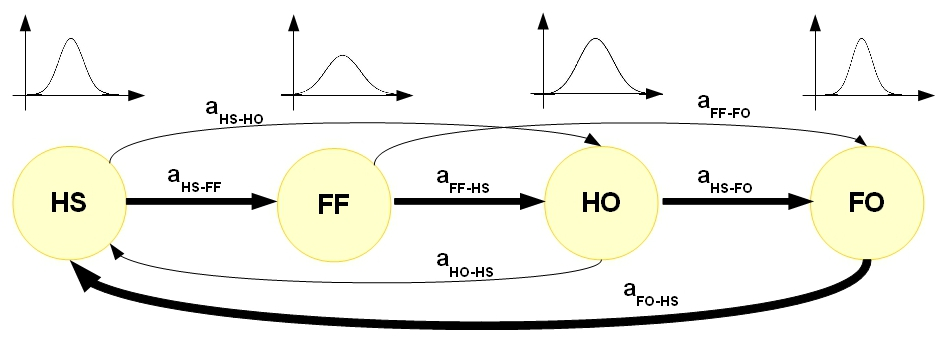
\includegraphics[width=1\textwidth]{imgs/HMM.jpg}
	\caption{Grafico del segnale di un giroscopio posizionato sul piede.}
	\label{fig:deamb_hmm}
\end{figure}


\begin{table}%
\centering
\begin{tabular}{|c|cc|}
\hline
\textbf{Stato} & \textbf{inizio} & \textbf{fine} \\
%\hline
\hline
$S_1$ & $t_{HS}$ & $t_{FF}$\\
%\hline
$S_2$ & $t_{FF}$ & $t_{HO}$\\
%\hline
$S_3$ & $t_{HO}$ & $t_{FO}$\\
%\hline
$S_4$ & $t_{FO}$ & $t_{HS}$\\
\hline	 
\end{tabular}
\caption{Le quattro fasi della deambulazione e gli eventi (tempo iniziale e finale) che li definiscono.}
\label{tab:4_fasi_deambulazione}
\end{table}
Per semplicit� si pu� indicare uno stato $S_i$ con l'evento da cui ha inizio, ad esempio con lo stato $HS$ indico lo stato $S_1$.


\section{Addestramento del Modello}

\section{Parametri ottenuti}